\chapter{Felhasználói dokumentáció} % User guide
\label{ch:user}

\section{Rendszerkövetelmények}

A program futtatásához szükséges, hogy a \textit{pgrep} program telepítve legyen, és a helye hozzá legyen adva a \textit{PATH}-hoz. Ez Ubuntu 20.04 LTS operációs rendszer esetén alapértelmezett.

\section{Telepítés és indítás}

A program fordításához az alábbiakra van szükség:
\begin{compactenum}
	\item GHC, legalább 8.6.5 verzió (valószínűleg korábbiakra is működik)
	\item Haskell csomagok: \textit{base, cereal, fgl, ghcid, gtk2hs, microlens-platform, parsec, split, unliftio}, illetve ezen csomagok függőségei. 
\end{compactenum}

A fentiek megléte esetén a program az alábbi paranccsal fordítható: 

\textit{ghc Main.hs -o insertNameHere}

\textit{insertNameHere} helyére írható a futtatható állomány kívánt neve. Az alkalmazás az így kapott futtatható állomány futtatásával indítható el. Fontos, hogy az \textit{Empty.hs} fájl a futtatható állománnyal egy mappában helyezkedjék el, hogy a kiértékelés az ezen dokumentációban leírt módon működjék. \textbf{EZ AM FULL GÁZ, KONFIGURÁLHATÓVÁ KÉNE TENNI.}

\section{A felhasználói felület áttekintése}

\begin{figure}[H]
	\centering
	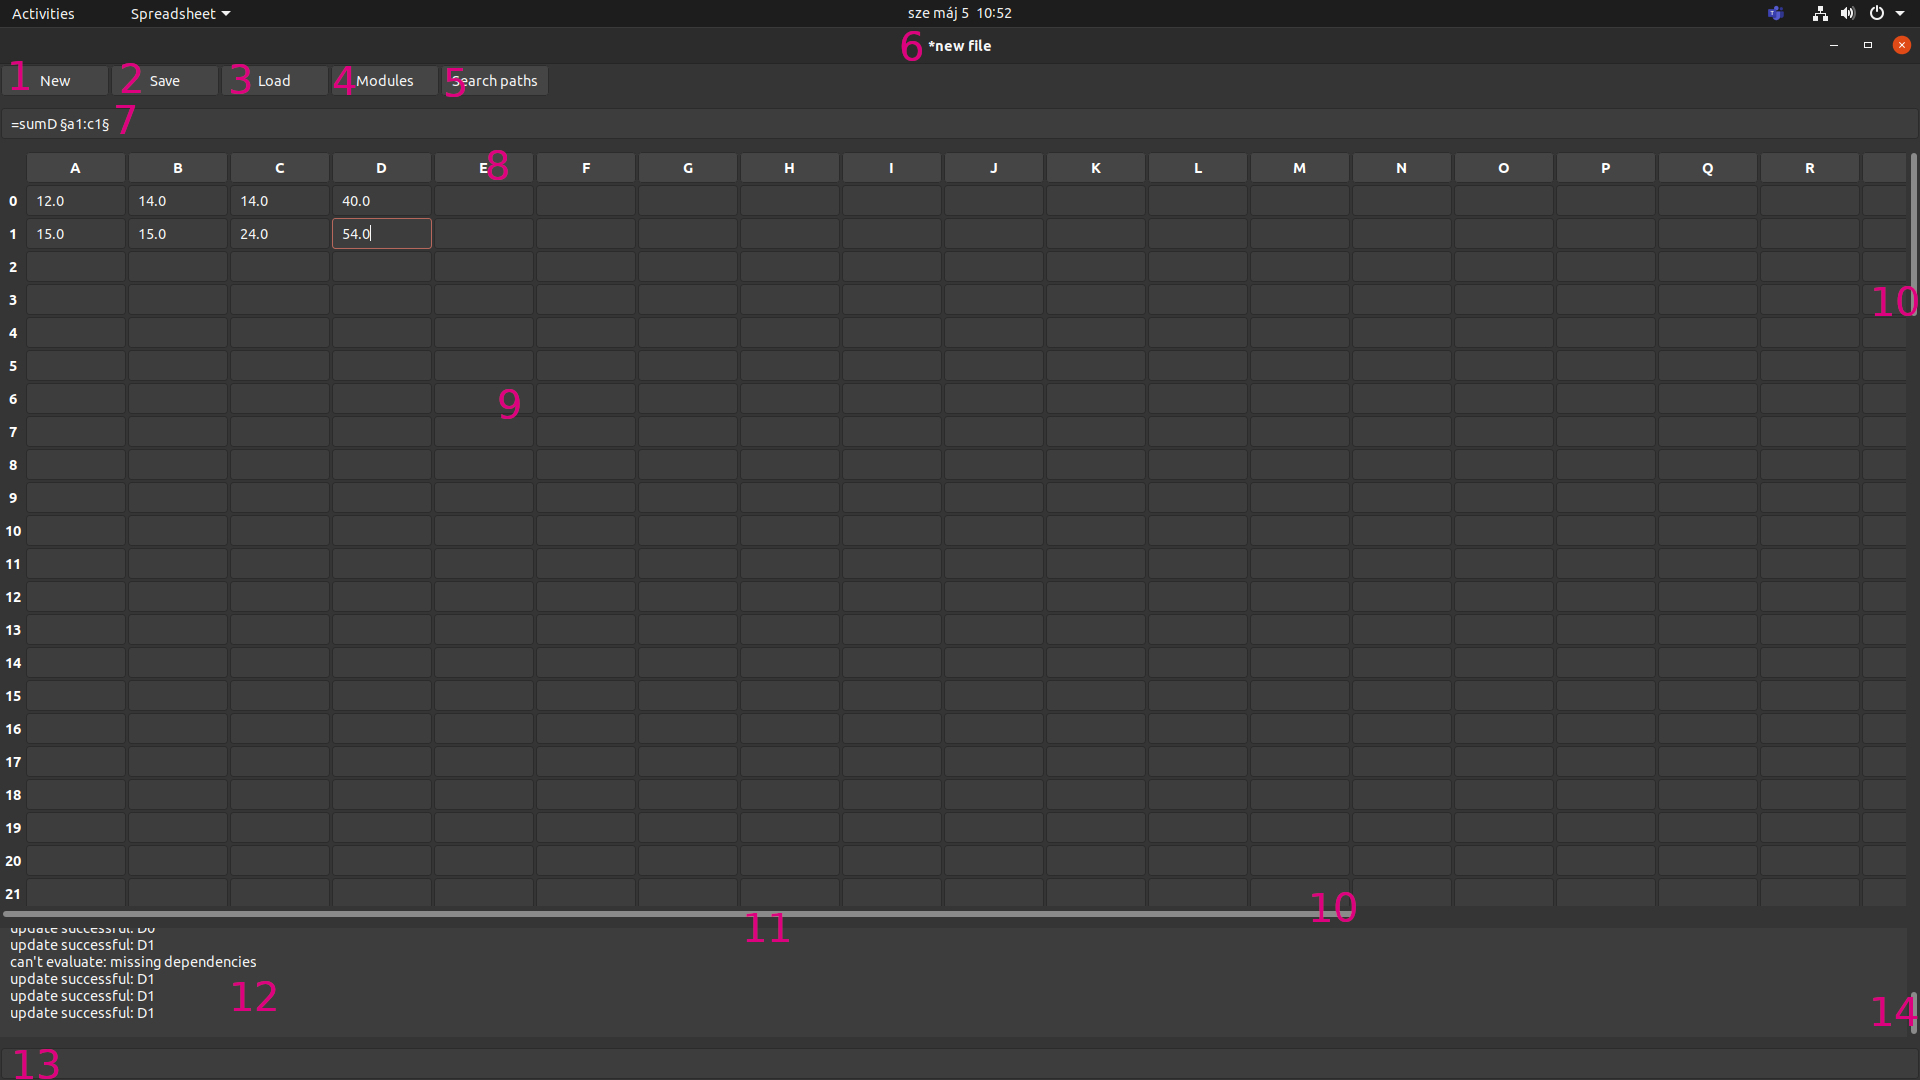
\includegraphics[width=\textwidth]{gui}
	\caption{A felhasználói felület}
	\label{fig:gui}
\end{figure}

\begin{compactenum}
	\item Ezzel a gombbal lehet új fájlt létrehozni. Ekkor a számolótábla üres lesz.
	\item Ezzel a gombbal lehet elmenteni a számolótábla aktuális állapotát. A fájl az alkalmazás saját \textit{.fsandor} kiterjesztésében kerül mentésre.
	\item Ezzel a gombbal lehet fájlt betölteni.
	\item Ezzel a menüponttal lehet beállítani a háttérben futó GHCi-be betöltendő modulok listáját. A felugró szövegmező minden sora egy modult jelent.
	\item Ezzel a menüponttal lehet beállítani, hogy az alapértelmezett útvonalakon kívül hol keresse a GHCi a betöltendő modulokat. Minden sor egy elérési útvonalat jelent. Az elérési útvonal lehet abszolút (ez utóbbi a javasolt) vagy relatív a futtatható állomány helyéhez képest.
	\item A betöltött fájl neve. Ha épp nincs elmentve a számolótábla, a "*new file" szöveg jelenik meg. Ha a betöltött fájl neve előtt szerepel egy "*", az azt jelenti, hogy a legutóbbi mentés óta történt módosítás.
	\item Kódszerkesztő. Ebbe a sorba lehet kódot írni az aktuálisan kijelölt cellához. A kijelölt cella az a cella, amelyre a felhasználó legutóbb kattintott. A beírt kód akkor kerül kiértékelésre, ha a felhasználó egy másik elemre kattint vagy leüti az entert.
	\item A számolótábla. A cellába beírt kód akkor kerül kiértékelésre, ha a felhasználó egy másik elemre kattint vagy leüti az entert.
	\item A log mutatja a végrehajtott akciók (pl. cella kódjának átírása, GHCi query eredménye) eredményét. Jobb oldalt görgethető.
	\item Az alkalmazáshoz tartozó parancssor. A beírt parancs akkor kerül kiértékelésre, ha a felhasználó leüti az entert.
\end{compactenum}

\section{A parancssorban használható parancsok}

\subsection{Kifejezés kiértékelése GHCi-ban}

A program a cellák kódjának kiértékeléséhez a háttérben egy GHCi példányt futtat. Jelölje a $\_$ a szóköz karaktert és $C$ az összes karakterek halmazát. Amennyiben a beütött parancs $\_^+g\_^+C^*$ alakú, a "g"-t követő szóközök utáni részstring kiértékeltetik a GHCi-ban. A kiértékelés eredménye megjelenik log üzenetként. 

Ezen parancs segítségével lehetséges modulokat importálni és bindingokat létrehozni a GHCi által használt IO monádban. Azonban minden egyes cellakiértékelés előtt a bindingok elvesznek, a betöltött modulok pedig azok lesznek, amelyek a "Modules" menüpontban meg lettek adva. Így a gyakorlatban a GHCi ezen funkciói nem használhatók.

\section{A cellákba írható kifejezések}

\subsection{A kifejezések lehetséges típusai}

Egy cella tartalma négyféle lehet: üres cella, szám, szöveg vagy formula. A cellába beírt kifejezés pontosan akkor formula, ha az első karaktere "=". Amennyiben az első karakter nem "=", és a beírt szöveg értelmezhető tizedestörtként, annyiban a cella tartalma számként kerül értelmezésre. Minden más esetben a cella tartalma egy string. Példák:
\begin{itemize}
	\item Szám: "0.12", "11"
	\item Formula: "=sum [1..10]", "=§a0§+sumD §a2:b4§"
	\item String: " =sum [1..10]", "alma", ".12"
\end{itemize}

A kiértékeléshez a

\end{enumerate}